\documentclass[a4paper,11pt]{article}
\usepackage{a4wide}
\usepackage{geometry}
  \geometry{paper=a4paper,top=2.2cm,bottom=2.9cm}
   \geometry{right=2.3cm,left=2.3cm}
% Feynman diagrammen
\usepackage{feynmp}
\unitlength = 1mm
% Afbeeldingen
\usepackage{graphicx} % afbeeldingen
\usepackage{subfigure} % pakket voor het gebruiken van sub-figuren
\usepackage{float} % laat toe [H] te gebruiken bij plaatsen figuren
% Taal
\usepackage[dutch]{babel}
%\hyphenation{}
% De formules
\usepackage{amssymb, amsmath} % wiskunde
\numberwithin{equation}{section} % (#.#) i.p.v. (#)
% xetex
\usepackage{fontspec}
\usepackage{xunicode}
\usepackage{xltxtra}
\setromanfont[Mapping=tex-text]{Calibri}
% appendix
\usepackage{appendix}

\title{Studie van parton-saturatie effecten in de transversale energiestroom en $F_L$ bij elektron-proton interacties aan de LHeC}
\author{Ruben Van Boxem}

\begin{document}

% titelpagina
\fontsize{12pt}{14pt}\selectfont

\begin{center}


\includegraphics[height=3cm]{Afbeeldingen/UA.eps}

\vspace{1cm}

\fontsize{14pt}{17pt}\selectfont
% De Faculteit:
\textsc{Faculteit Wetenschappen} \\
\textsc{Departement Fysica}
\fontsize{12pt}{14pt}\selectfont
\vspace{0.3cm}

\vspace{1.2cm}

%Het academiejaar: aanpassen!
Academiejaar 2009--2010

\vspace{2.8cm}

\fontsize{17.28pt}{21pt}\selectfont

% De titel van de thesis:
\textsc{Studie van parton-saturatie effecten in de transversale energiestroom en $F_L$ bij elektron-proton interacties aan de LHeC}

\fontseries{m}
\fontsize{12pt}{14pt}\selectfont

\vspace{3cm}

% De auteur van de thesis:
Ruben \textsc{Van Boxem}	

\vspace{2cm}

Promotor: Prof. Dr Pierre \textsc{Van Mechelen}\\
Copromotor: Krzysztof \textsc{Kutak} \\
\vspace{2cm}
\end{center}
% De functie van de thesis:
Proefschrift voorgedragen tot \\
het behalen van de graad van\\
\textsc{Bachelor in de Fysica}

\thispagestyle{empty}
\newpage

\section*{Dankwoord}
Ik wil enkele mensen in het bijzonder danken voor de ontelbare uren die ze in mij en dit werk hebben gestoken:
\begin{itemize}
  \item mijn promotor, Prof. Dr. Pierre Van Mechelen,
  \item mijn copromotor en die-hard begeleider, Dr. Krzysztof Kutak,
  \item al de mensen van de EDF groep aan de UA die onrechtstreekse hulp hebben geboden
\end{itemize}
Daarnaast, een algemene dank u wel aan de volgende mensen:
\begin{itemize}
  \item de hele 3de bachelor fysica (en zij die daar zouden moeten bijhoren),
  \item mijn vader en moeder voor de onmisbare steun,
  \item Pieter Taels in het bijzonder omdat hij ook tijdens de vakantie bij mij op de unief kwam werken,
  \item en iedereen die van zichzelf vindt dat hij/zij hier in dit lijstje had moeten staan en ik al dan niet bewust vergeten ben.
\end{itemize}

\thispagestyle{empty}
\newpage
\fontsize{11pt}{14pt}\selectfont

\section*{Summary}
A theoretical study of saturation and its effects in the transverse energy flow for proton-electron collisions is made.
A short introductory text on deep inelastic scattering and general QCD theory serves as an intro to the concepts important in this field.
Concepts like structure functions, resummation, running coupling constant, etc. are introduced in a natural way.
Starting from a simple electron-nucleus collision, through several layers of scaling violations and QED interactions, a summary is given of the advances in theory trying to incorporate the newest experimental findings (the latest being HERA), which keep penetrating deeper into the core of fundamental interactions.
Different types of higher order corrections to the simplest parton model are described, and their assumed shortcomings for the LHeC kinematic region are shown.
Saturation, a very promising approach to naturally correct for the currently predicted infinities in QCD at low $x$, is introduced by means of the corrected (seccond order) BFKL equation, the BK equation.
Saturation effects as described by the Golec-Biernat-Wüsthoff model are studied in the structure functions of the proton, and the directly measurable transverse energy flow of high energy, low $x$ electron-proton collisions.

\thispagestyle{empty}
\newpage

\tableofcontents
\thispagestyle{empty}
\newpage

\section{Diepe inelastische verstrooiing}
      \paragraph{}
Om de diepere structuur van een object zoals het proton te bestuderen, kan men elektron verstrooiing gebruiken.
Door middel van een elektron met hoge energie op een proton te laten botsen kan men de onderliggende samenstelling van het proton bestuderen.
Een proces dat zich hier goed voor leent, heet DIS, oftewel \textit{Deep Inelastic Scattering}. In figuur \ref{fig:DIS} wordt een DIS proces schematisch weergegeven.
\begin{figure} [H]
  \begin{center}
    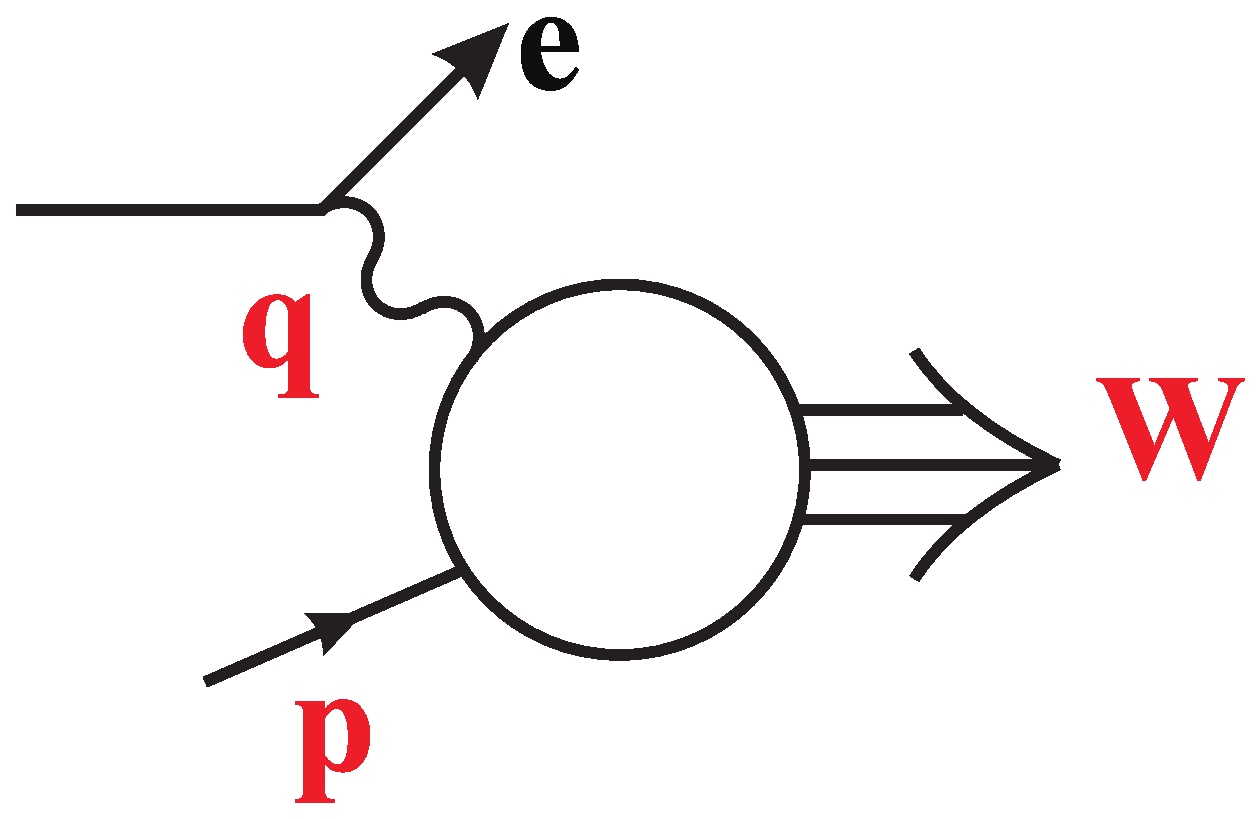
\includegraphics[width=.33\textwidth]{Afbeeldingen/DIS.eps}
    \caption{Elektron-proton verstrooiing.
Het elektron zendt een boson uit dat het proton “onderzoekt".
$P$ is de vierimpuls van het inkomend proton, $W$ is de invariante massa van het uitgaande systeem (zonder elektron), $q$ is de overgedragen vierimpuls. \cite{Martin}}
   \label{fig:DIS}
  \end{center}
\end{figure}
 In wat volgt wordt M gedefinieerd als de massa van het proton. Men spreekt van DIS processen als $Q^2 \gg M^2$ (“diep”) en $W^2 = (P+q)^2 \gg M^2$ (“inelastisch”).
$Q^2$ wordt ook angeduid als de virtualiteit van het foton.
Omdat de waarde van $q^2$ negatief is, wordt vaak volgende variabele ingevoerd: $Q^2 :=-q^2 > 0$.  Dit is een ruimteachtige vierimpuls, dus er bestaat een stelsel waar de energie van het virtuele foton nul is en dus de impuls gelijk aan $Q^2$. In dit stelsel is de golflengte van het het foton van de grootteorde van $1/Q$.
Dit wil concreet zeggen dat als de overgedragen impuls verhoogt, de golflengte van het foton en dus de grootte van de deeltjes waarmee het interageert, kleiner wordt.

      \paragraph{}
Men kan twee soorten DIS interacties onderscheiden: neutrale en geladen stroom (respectievelijk NC en CC). De Feynman diagrammen worden weergegeven in figuur \ref{fig:NC-CC}.
\begin{figure} [H]
  \centering
  \subfigure[NC interactie met uitwisseling van een foton of $Z$ boson.]{
  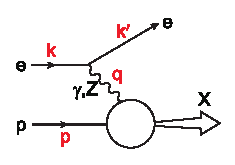
\includegraphics[width=.33\textwidth]{Afbeeldingen/NC.eps}
  \label{fig:NC}
  }
  \subfigure[CC interactie met uitwisseling van een $W^\pm$ boson.]{
  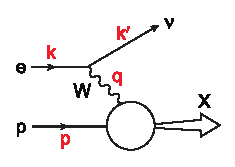
\includegraphics[width=.33\textwidth]{Afbeeldingen/CC.eps}
  \label{fig:CC}
  }
  \caption{Soorten DIS. \cite{Martin}}
  \label{fig:NC-CC}
\end{figure}

      \paragraph{}
In wat volgt wordt beschreven wat er gebeurt als men $Q^2$ systematisch verhoogt.

  \subsection{Breking van schaalinvariantie}
    \paragraph{Elektron-kern verstrooiing}
Stel dat een elektron verstrooid wordt op een atoomkern (bestaande uit meerdere nucleonen).
Als $\lambda \gg d_\text{kern}$, ziet het foton de kern als een puntdeeltje en wordt het elastisch verstrooid op een puntdeeltje met de lading van de kern.
Als $\lambda \ll d_\text{kern}$, dringt het foton diep door in de kern en kan het verstrooid worden op een proton in de kern.
Men spreekt hier van diep inelastische elektron-kern verstrooiing, en men kan het volgende schrijven:
\begin{equation}
x_N = \frac{M}{M_N} \left( \frac{Q^2}{2M\nu} \right) = \frac{1}{A}
\end{equation}
waarbij $M_N$ de massa van de kern is, $M$ de massa van het proton, $\nu$ de frequentie van het foton en $A$ het aantal nucleonen in de kern.
De laatste gelijkheid geldt omdat het elektron elastisch interageert met een geheel nucleon.
Als men de werkzame doorsnede van deze processen zou uitzetten t.o.v. $x_N$, ziet men een duidelijke verschil tussen de gevallen waar $\lambda \gg d_\text{kern}$ en die waar $\lambda \ll d_\text{kern}$.
Dit fenomeen heet \textit{breking van schaalinvariantie}, waarbij de waargenomen werkzame doorsnede blijkbaar afhangt van de grootte van de schaal, $Q^2$.

      \paragraph{Elektron-proton verstrooiing}
Zolang dat $\lambda \gg d_\text{proton}$, ziet het foton het proton als puntdeeltje. Het wordt elastisch verstrooid door het proton.
Als $Q^2$ zo groot is dat $\lambda \ll d_\text{proton}$, wordt er opnieuw ``ingezoomd", waarbij het foton nu de bouwstenen van het proton kan “zien" (i.e. ermee kan interageren).
Het foton ziet dus de 3 quarks als puntdeeltjes en men spreekt van diep inelastische elektron-proton verstrooiing.
Kinematisch geldt het volgende (zie appendix \ref{app:DIS}):
\begin{equation} \label{eq:Bjorkenx}
x = \left( \frac{Q^2}{2p\cdot q} \right)
\end{equation}
$x$ wordt aangeduid als de “Bjorken schaalvariabele".
De waarschijnlijkheid van zo'n proces worden dus enkel en alleen bepaalt door $x$ en niet $Q^2$ en $p\cdot q$ afzonderlijk.

      \paragraph{Breking van schaalinvariantie}
In volgorde van stijgende $Q^2$ heeft men dus voor de werkzame doorsnede:
\begin{itemize}
  \item\textit{kern}schaling met een piek op $x_N=1$
  \item  breking van schaalinvariantie
  \item \textit{proton}schaling met een piek \textit{rond} $x \sim 1$
  \item breking van schaalinvariantie
  \item \textit{Bjorken}schaling met een \textit{uitgesmeerde} piek rond $x \sim 1/3$ (3 quarks)
\end{itemize}
Als men $Q^2$ blijft vergroten, verwacht men logischerwijs nogmaals een breking van schaalinvariantie te zien, en deze worden ook geobserveerd.
De schijnbare breking van schaalinvariantie ligt in lijn met de voorspellingen van QCD, de theorie van de sterke wisselwerking.
Deze laatste breking van schaalinvariantie is dus niet te wijten aan een substructuur van quarks, maar kan verklaard worden door quark-gluon interacties in QCD.

  \subsection{Zeequarks, gluonen en $\alpha_S$}
Quarks blijken niet uit een diepere structuur te bestaan (zodat er niet opnieuw een breking van schaalinvariantie optreedt).
In plaats van een diepere quark structuur, beschrijft QCD het proton als 3 valentiequarks (de klassieke $u u d$ combinatie) plus een willekeurig aantal zeequarks ($q\bar{q}$ paren).
Het foton ziet naast drie puntdeeltjes ook een zee van quarks.
Zeequarks ontstaan uit gluonen ($g\rightarrow q\bar{q}$) die zelf uitgestraald worden door andere quarks ($q\rightarrow gq$).
Het feit dat er extra deeltjes moeten bestaan in een proton volgt ook uit de experimentele waarneming dat slechts de helft van de impuls van het proton gedragen wordt door z’n quarks (zee- en valentiequarks).
De breking van schaalinvariantie kan dus verklaard worden uit het gedrag van de samenstellende partonen in een proton.
Een enkelvoudige quark blijkt bij hogere $Q^2$ te bestaan uit $q g/q q\bar{q}$.
De impuls van het quark wordt dus verdeeld over meer deeltjes.
Het aantal partonen neemt toe, en tegelijkertijd neemt de fractionele impuls $x$ af.
Omgekeerd, bij hogere $x$ vermindert het aantal partonen met stijgende $Q^2$.
Daarnaast zal bij kleine $x$ dus het aantal partonen groter worden met stijgende $Q^2$.
Er treedt dus breking van schaalinvariantie op omdat elk parton (quark of gluon) bij een grotere waarde van $Q^2$, een kleiner deel  $x$ van de impuls $P$ van het proton zal dragen.
Deze breking van schaalinvariantie heeft volgende vorm:
\begin{equation}
\alpha_S R \ln{\left( \frac{Q^2}{\mu^2}\right)}
\end{equation}
Hier is $R$ een observabele en $\mu$ de renormalisatie schaal.
Bovenstaande formule geeft een bijdrage van een eerste orde term in $\alpha_S$ (zie sectie \ref{sec:DGLAP}).
Dit zal duidelijk worden in de context van sectie \ref{sec:Observabelen}.
Merk op dat in tegenstelling tot de vorige brekingen van schaalinvariantie, deze logaritmisch is, wat bijzonder moeilijk te meten was toen deze ontdekking werd gedaan.

  \subsection{$\alpha_S$}
De sterke wisselwerking (met koppeling $\alpha_S$) is fundamenteel ingewikkelder dan bijvoorbeeld de elektromagnetische (met koppeling $\alpha$).
Dit verschil in complexiteit stemt van de wiskundige abstractie die gemaakt wordt van de fysische interactie.
De elektromagnetische wisselwerking (QED) vindt zijn oorsprong in de locale invariantie voor fasetransformaties van de velden veroorzaakt door elektrische lading.
Deze eigenschap leidt tot de symmetrie van de U(1) groep: QED is een U(1) lokaal Abelse ijktheorie.
QED heeft dan ook een enkel interactie boson, namelijk het foton.
QCD daarentegen, is een SU(3) niet-Abelse ijktheorie, die lokaal invariant is voor fasetransformaties van de velden veroorzaakt door de 3 kleurladingen.
Dit geeft onder andere aanleiding tot 8 (+1 singlet) verschillende interactie bosonen, namelijk de gluonen.
Om het cruciale verschil te illustreren, wordt eerst kort QED geschetst, om daarna (de problemen van) QCD beter te kunnen begrijpen.

    \subsubsection{QED en $\alpha$} \label{sec:QED}
Om de vorm en het gedrag van de sterke koppeling te begrijpen, is het handig om eerst kort de koppeling in QED ($\alpha = e^2/4\pi$) te bekijken.
De processen die bijdragen aan een interactie van een foton met een enkel elektron worden in figuur \ref{fig:QED} weergegeven.
\begin{figure} [H]
  \begin{center}
    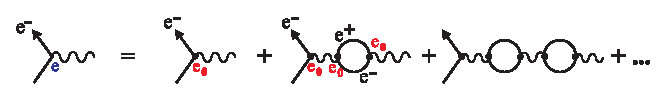
\includegraphics[width=.66\textwidth]{Afbeeldingen/QED.eps}
    \caption{Feynman diagrammen van de processen die bijdragen tot de interactie tussen een foton en een elektron. $e_0$ duidt hier op de naakte lading van het elektron.}
   \label{fig:QED}
  \end{center}
\end{figure}
De lading van een kaal elektron wordt afgeschermd door de “polarisatie van het vacuüm”, waardoor het foton extra $e^+ e^-$-paren “voelt”.
Hoe korter de golflengte van het foton, hoe meer $e^+ e^-$-paren het zal voelen.
Dit zorgt ervoor dat $\alpha$ toeneemt met $Q^2$.
De normalisatie van $\alpha$ komt uit vergelijking met experimentele data.
Algemeen kan men de elektromagnetische koppelingsfactor schrijven als volgt.
\begin{equation}
\alpha(Q^2) = \alpha_0 \left[ 1+ \frac{\alpha_0}{3\pi} \ln{\frac{Q^2}{M^2}} + \left( \frac{\alpha_0}{3\pi} \ln{\frac{Q^2}{M^2}} \right)^2 +\hdots \right]
\end{equation}
De \textit{loops} in de hogere orde Feynman diagrammen kunnen een oneindige bijdrage hebben indien er geen \textit{cut-off} waarde voor de \textit{loop}impuls wordt opgelegd.
Er wordt dus een renormalisatieschaal ingevoerd om de eindigheid te garanderen.
QED beschrijft dus het verloop van $\alpha$, en het experiment geeft het een absolute waarde.
Als men de waarde van $\alpha$ kent voor een waarde $\mu^2$, volgt hieruit de waarde van $\alpha$:
\begin{equation} \label{eq:alpha}
\alpha( Q^2 ) =\frac{\alpha(\mu^2)}{1-\frac{\alpha(\mu^2)}{3\pi} \ln{\frac{Q^2}{\mu^2}}}
\end{equation}

    \subsubsection{QCD en $\alpha_S$}
\begin{figure} [H]
  \begin{center}
    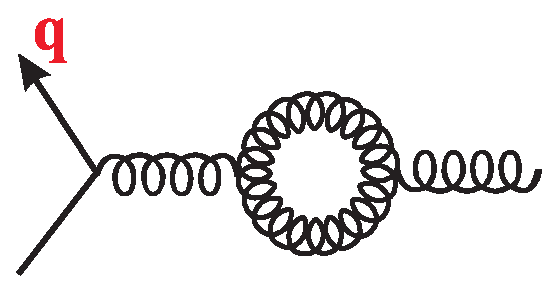
\includegraphics[scale=.33]{Afbeeldingen/GluonLoop.eps}
    \caption{Extra diagram bij QCD, dat voor \textit{antiscreening} zorgt. \cite{Martin}}
   \label{fig:GluonLoop}
  \end{center}
\end{figure}
QCD heeft nog een extra diagram dat de situatie iets moeilijker maakt, namelijk een vertex van drie gluonen, en bijhorende loop van pure gluonen (zie figuur \ref{fig:GluonLoop}).
Een fermion loop brengt afscherming van de (kleur)lading met zich mee (zie \ref{sec:QED}).
Een gluon loop zorgt voor \textit{antiscreening}, waardoor  $\alpha_S$ stijgt naarmate $Q^2$ kleiner wordt.
Dit volgt uit de uitdrukking voor $\alpha_S$, analoog aan \eqref{eq:alpha}:
\begin{align}
\alpha_S( Q^2 ) &=\frac{\alpha(\mu^2)}{1+b_0 \alpha(\mu^2) \ln{\frac{Q^2}{\mu^2}}} \\
\text{met} b_0 &= \frac{-n_f}{6\pi} + \frac{33}{12\pi} \notag
\end{align}
Hier is $n_f$ het aantal soorten quarks die verondersteld worden.
Hier heeft de coëfficiënt (hier $b_0$) dus het tegengestelde teken, waar de tegenstelling tussen QED en QCD uit volgt.
Dit kan men herschrijven zodat de enige vrije parameter van QCD naar voor komt (zie bijvoorbeeld \cite[sectie 6.6]{Bettini}):
\begin{align} \label{eq:runningAlphaS}
\alpha_S(Q^2) = \frac{12\pi}{(33-2n_f) \ln{\frac{|Q|^2}{\lambda_\text{QCD}}}}
\end{align}
Waarbij $\lambda_\text{QCD}$ de fundamentele parameter in QCD is, die uit experimentele metingen wordt bepaald.
$\lambda_\text{QCD}$ hangt af van het aantal soorten quarks die bijdragen aan het proces $n_f$ (\cite[sectie 6.6]{Bettini}):
\begin{align}
\lambda_\text{QCD} = \mu^2 exp \left[ \frac{-12\pi}{(33-n_f) \alpha_S(\mu^2)} \right]
\end{align}
Voor drie en vier quarksoorten is $\lambda_\text{QCD}$ respectievelijk ongeveer gelijk aan 400 en 200 MeV.
Waarbij $\mu^2$ een schaalvariabele is waarvoor de koppeling gekend is.
$\lambda_\text{QCD}$ is zeer invloedrijk in verdere QCD berekeningen.
Als de energie kleiner is dan $\lambda_\text{QCD}$, is $\alpha_S$ groot en kan men geen perturbatieve berekeningen uitvoeren.
Daarbij komt dat $\alpha$ en $\alpha_S$ niet rechtstreeks gemeten kunnen worden, maar enkel door een theoretische berekening uit experimentele data kunnen worden afgeleid.
$\alpha_S$ zal dan bijgevolg minder nauwkeurig zijn, wegens zijn relatieve grootte.

    \subsubsection{Renormalisatiegroep vergelijking}
Omdat de keuze van $\mu^2$ in een berekening onmogelijk de gemeten waarde van een observabele kan beïnvloeden, moet er expliciet voor gezorgd worden door middel van de \textit{renormalisation group equation}:
\begin{align} \label{eq:RGE}
\frac{d R}{d\ln{\mu^2}} &= \left(\frac{\partial}{\partial \ln{\mu^2}} + \frac{\partial \alpha_S}{\partial \ln{\mu^2}} \frac{\partial}{\partial \alpha_S} \right) R \\
\Rightarrow &R(Q^2/\mu^2, \alpha_S(Q^2)) = R(1,\alpha_S(Q^2)) \notag
\end{align}
Dit laatste betekent dat de twee afhankelijkheden (op $Q^2/\mu^2$ en $\alpha_S(\mu^2)$) eigenlijk maar een enkele zijn, namelijk het verloop van $\alpha_S(Q^2)$. Voor een uitwerking van de dubbele pijl in \eqref{eq:RGE} zie appendix \ref{app:RGE}).

    \subsubsection{QCD observabelen} \label{sec:Observabelen}
      \paragraph{}
Elke observabele kan in perturbatieve QCD ontwikkeld worden in machten van $\alpha_S$.
Bijkomende factoren zullen gevormd worden door logaritmes van $Q^2$ en bij lage $x$, $1/x^2$.
Omdat een observabele per definitie een eindig getal moet zijn, moeten de op eerste zicht divergente reeksen in $\alpha_S$ gehersommeerd worden.
Deze hersommatie kan enkel in speciale gevallen gebruikt worden, en alle tot nu toe bekende vormen zijn enkel in een bepaald regime (van $Q^2$ en/of $x$) geldig.
Omdat de exacte techniek op z’n minst moeilijk en zeer technisch is, worden hieronder enkel een beschrijving van de benaderingen en hun resultaten besproken. (\cite[sectie 9.5.2]{Barone})

      \paragraph{LLA}
\textit{Leading $\ln{Q^2}$ approximation}, waar de termen van de vorm $\alpha_S^n \ln^n{Q^2}$ gehersommeerd worden:
\begin{align} \label{eq:LLA}
R = \sum_n \alpha_S \ln^n{Q^2} \left( \sum_{k=n}^0 \ln^k{\frac{1}{x}} \right)
\end{align}
Dit leidt tot de DGLAP evolutievergelijkingen, die de evolutie van een observabele beschrijft in $Q^2$ bij “normale” $x$.
Indien ook termen van de vorm $\alpha_S^n \ln^{n-1}{Q^2}$ behouden blijven, krijgt men \textit{next-to leading $\ln{Q^2}$ approximation} en bijgevolg de NLLA DGLAP vergelijkingen.

      \paragraph{DLLA}
\textit{Double leading log approximation} duidt op het feit dat termen van de vorm $\alpha_S \ln^n{Q^2} \ln^n{\frac{1}{x}}$ behouden blijven:
\begin{align}
R = \sum_n \alpha_S \ln^n{Q^2} \ln^n{\frac{1}{x}}
\end{align}

      \paragraph{LL$_x$A}
In de praktijk zal voor heel lage $x$, $Q^2$ klein zijn, en men enkel de termen van de vorm $\alpha_S^n \ln^n{\frac{1}{x}}$ behoudt. Zo krijgt men de \textit{leading $\ln{\frac{1}{x}}$ approximation}:
\begin{align}
R = \sum_n \alpha_S \ln^n{\frac{1}{x}} \left( \sum_{k=n}^0 \ln^k{Q^2} \right)
\end{align}
\eqref{eq:LLA} en bovenstaande vergelijking zijn symmetrisch ten opzichte van $Q^2$ en $1/x$. Deze laatste leidt ook tot een veel bestudeerde BFKL evolutievergelijking.

      \paragraph{Parton dichtheden}
Een probleem in de recente resultaten van DGLAP berekeningen tot \textit{next-to next-to leading order}, is het opblazen van de parton dichtheden in een proton voor zeer kleine $x$.
In figuur \ref{fig:PD} staat voor twee verschillende schalen $Q^2$ getoond wat de dichtheden van de verschillende partons (gluonen en (zee)quarks) in het proton zijn.
Als dit verloop blijft doorgaan, zullen dichtheden optreden die niet meer fysisch zijn (unitariteit is niet meer geldig), waardoor de kans om met een parton te botsen groter kan zijn dan 1.
\begin{figure} [H]
  \begin{center}
    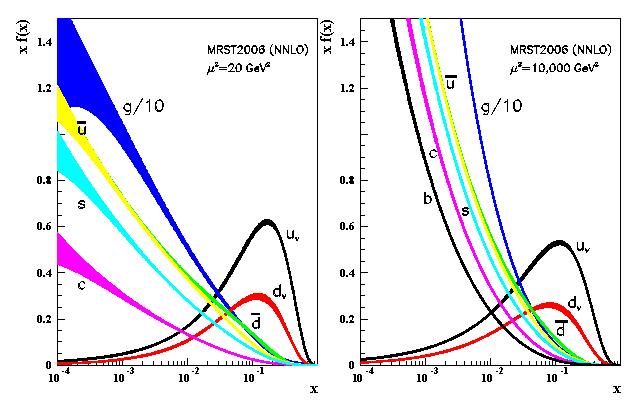
\includegraphics[scale=1]{Afbeeldingen/PD.eps}
    \caption{Dichtheden van de verschillende partonen in een proton voor twee verschillende schalen $Q^2$. Voor kleine $x$ gaan de gluonen sterk domineren. Voor relatief grote $x$-waarden vindt men de klassieke $uud$ combinatie terug, met de gluonen en zeequarks sterk onderdrukt. Veer zeer kleine waarden van $x$ blazen de dichtheden van de zeequarks en vooral de gluonen op.\cite{Martin}}
   \label{fig:PD}
  \end{center}
\end{figure}

    \subsubsection{DGLAP en BFKL}
Evolutievergelijkingen geven het verband tussen een grootheid (bijvoorbeeld een dichtheidsfunctie van quarks of gluonen) bij een (bijna) willekeurige waarde van $Q^2$ of $x$ en de waarde van de grootheid bij een bekende $Q_0^2$ of $x_0^2$.
DGLAP en BFKL geven elk een andere fysische interpretatie van de uiteindelijke interactie.
Het beeld dat het vaakst gebruikt wordt om de uitgestraalde gluonen weer te geven, is de gluonladder.
Om de extra partonen die blijken aanwezig te zijn in het proton te beschrijven, wordt vanuit een (valentie)quark in het proton een gluon uitgestraald, dat op zijn beurt een onbepaald aantal gluonen uitstraalt. Deze ladder van gluonen wordt weergegeven in figuur \ref{fig:GluonLadder}.
\begin{figure} [H]
  \begin{center}
    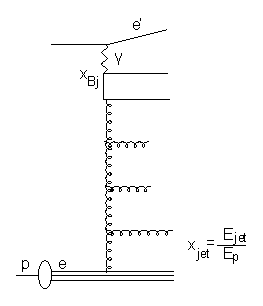
\includegraphics[scale=1]{Afbeeldingen/GluonLadder.eps}
    \caption{Een DIS interactie, met weergegeven gluonladder. Aan het elektron heeft het interagerend parton een welbepaalde waarde van $x$, waardoor er gesommeerd moet worden over alle gluonladders die zo’n finale $x$ opleveren. Naast de centrale DIS interactie treden er ook voorwaartse jets op, die veel informatie kunnen opleveren over de gluonladder zelf. \cite{Kiesling}}
   \label{fig:GluonLadder}
  \end{center}
\end{figure}

      \paragraph{DGLAP} \label{sec:DGLAP}
De DGLAP vergelijkingen kunnen gebruikt worden om de quark- en gluondichtheden voor een hogere waarde van $Q^2$ te berekenen, indien deze dichtheden bij een kleinere waarde $Q_0^2$ bekend zijn.
DGLAP is in eerste instantie (als lage orde benadering) enkel geldig voor voldoende grote $x$.
De $x$ afhankelijkheid is hier onbekend, en moet experimenteel worden vastgesteld.
Men kan DGLAP uitdrukken als de benadering waar de waarnemer ($Q^2$, de golflengte van het onderzoekend foton) en $x$ ingebouwd zit.
Er is dus geen verdere informatie over de inwendige detailstructuur van het proton meegegeven.
Als men figuur \ref{fig:GluonLadder} beschouwt, krijgt men in het DGLAP schema een sterke ordening in $\vec{k}_\perp$ voor opeenvolgende gluonemissies:
\begin{equation}
Q^2 \gg \vec{k}_\perp^2 \gg \vec{k}_{1\perp}^2 \gg \vec{k}_{2\perp}^2 \gg \hdots \gg \vec{k}_{n\perp}^2
\end{equation}
Daarnaast is er een normale ordening in $x$:
\begin{equation}
x < x_1 < x_2 < \hdots < x_n < 1
\end{equation}
Fysisch betekent dit dus dat de opeenvolgende gluonen een kleinere impulsfractie dragen van het oorspronkelijke parton en steeds meer afbuigen van de botsingsas.
Dit heeft grote implicaties voor de geproduceerde jets: de eerste jet, die dichter bij de as wordt uitgestraald, zal een grotere energie hebben, en de laatste (tweede of derde) zal een lagere energie hebben.

      \paragraph{BFKL}
De BFKL vergelijkingen doen net het omgekeerde: als de dichtheden bij een bepaalde waarde $x_0$ bekend is (hier moeten bepaalde aannames gemaakt worden, omdat bij lage $x$ niets exact berekend kan worden), kunnen e dichtheden berekend worden voor (bijna) willekeurige $x$.
Net zoals bij DGLAP de $x$-afhankelijkheid niet bekend was, blijft bij BFKL de $Q^2$-afhankelijkheid onbekend.
Deze benadering is dan ook enkel geldig voor kleine $x$, en is niet toepasbaar bij grote $Q^2$.
BFKL kan men beschouwen als de benadering waar naast de $x$-afhankelijkheid, de inwendige structuur van het proton aan bod komt (door een $k_\perp$-afhankelijkheid, waar $k_\perp$ de transversale impuls is).
Net door dit verschil in hersommatie zal BFKL een sterke ordening in longitudinale impuls met zich meebrengen, en helemaal geen ordening in $\vec{k}_\perp$.
BFKL legt dan ook geen “beperkingen” op de jets en hun eigenschappen die volgen uit een $\vec{k}_\perp$-ordening.
Recent is er een hogere orde correctie uitgewerkt voor de BFKL hersommatie, namelijk de BK vergelijking.

      \paragraph{CCFM}
Naast BFKL en DGLAP bestaat ook een derde benaderingsmethode, die tracht tegelijkertijd de hoogste graadstermen in $\ln{Q^2}$ en $\ln{\frac{1}{x}}$ te hersommeren.
De eenvoudigste manier om CCFM uit te leggen zonder al te diep op details in te gaan is DLLA + een ordening in hoeken.
CCFM is veel meer dan enkel deze twee eigenschappen, maar dit volstaat hier.
De ordening in hoeken in de gluonladder duidt op het feit dat opeenvolgende gluonen steeds langs een grotere hoek worden uitgestraald als zijn voorganger, dus:
\begin{equation} \label{eq:HoekOrdening}
\theta \ll \theta_1 \ll \theta_2 \ll \hdots \ll \theta_n
\end{equation}
Appendix \ref{app:CCFM} gaat hier iets dieper op in.
Belangrijk om in te zien is dat CCFM probeert DGLAP en BFKL te unificeren, en gehoopt wordt dat CCFM dan ook voor een breder $x$-gebied geldig zal zijn.
De extra beperkingen die worden opgelegd vergemakkelijken de integraties niet, en het uitrekenen en werken met CCFM is dan ook moeilijker dan met DGLAP.

      \paragraph{Geldigheid}
Zoals al aan te voelen was, is elke vorm van evolutie maar geldig in een bepaald kinematisch gebied, net door de aannames die gemaakt werd bij het hersommeren van de reeks in $\alpha_S$.
In figuur \ref{fig:DGLAP-BFKL} wordt aangeduid wanneer welke vergelijkingen aangewezen zijn.
\begin{figure} [H]
  \begin{center}
    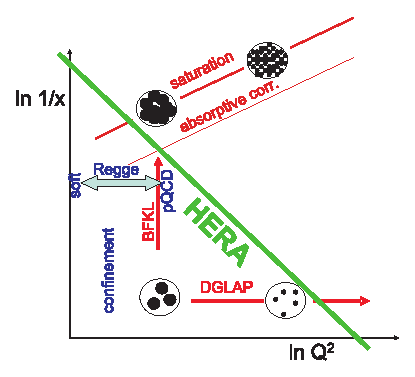
\includegraphics[scale=1]{Afbeeldingen/DGLAP-BFKL.eps}
    \caption{Schematische weergave van wat met verschillende benaderingen kan verwezenlijkt worden. Regge duidt op een gebied waar een pre-QCD theorie (Regge-theorie) geldig is. pQCD slaagt op perturbatieve QCD. \cite{Martin}}
   \label{fig:DGLAP-BFKL}
  \end{center}
\end{figure}
In figuur \ref{fig:DGLAP-BFKL} kan men ook een saturatielijn zien, die een theoretisch voorspelde grens vormt, waar saturatie van de partondistributies belangrijk zou worden (zie figuur \ref{fig:PD}).
De quark- en gluondistributies geven aanleiding tot structuurfuncties.
Deze waarschijnllijkheidsverdelingen beschrijven de structuur van een groter object (hier een proton) bij bepaalde $Q^2$ en $x$, in termen van hun samenstellende delen (hier partonen).
De groene “HERA”-lijn toont de grens van het kinematische gebied waarvoor metingen zijn uitgevoerd in HERA.
De LHeC zal (door zijn hogere botsingsenergie) buiten dit gebied kunnen meten en dus een duidelijke indicatie geven van fenomenen zoals saturatie die nu niet duidelijk kunnen worden gemeten.

    \subsubsection{Evolutievergelijkingen \textit{vs} experimentele data} \label{sec:QCDvsExperiment}
DGLAP is een vaststaande waarde die binnen de Elemtaire deeltjesfysica geldt als: \textit{it just works}.
Enkel recentelijk wordt omwille van metingen waarvan hieronder voorbeelden gegeven zijn, DGLAP meer en meer in twijfel getrokken.
DGLAP heeft nochtans (in het niet lage $x$ regime) krachtige en vooral juiste voorspellingen toegelaten, zoals HERA’s metingen van de sterke koppeling (zie figuur \ref{fig:SC}).
\begin{figure} [H]
  \begin{center}
    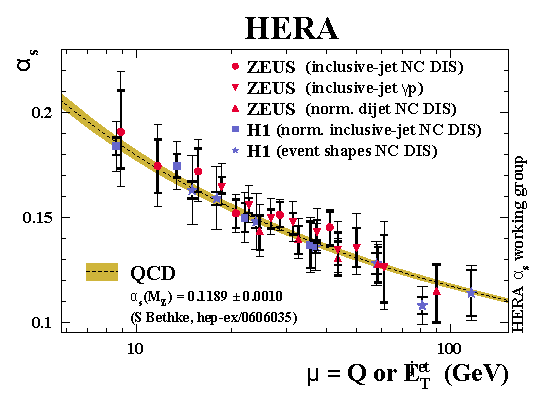
\includegraphics[scale=1]{Afbeeldingen/SC.eps}
    \caption{HERA metingen geplot tegenover de QCD voorspelling (DGLAP) voor de sterke koppeling. Merk op dat er over een heel groot $Q^2$-bereik een zeer goede overeenkomst is tussen theorie en experiment. \cite{Kiesling}}
   \label{fig:SC}
  \end{center}
\end{figure}

      \paragraph{Problematiek}
In HERA zijn verschillende metingen gedaan die met de nieuwste variaties van DGLAP en BFKL onvoldoende dicht bij de experimentele metingen raken.
Het betreft vooral metingen bij heel lage $x$, die niet goed beschreven worden door DGLAP omdat die termen net niet  of onvoldoende worden meegenomen.
BFKL/CCFM biedt in zijn pure vorm een mooi toekomstperspectief, en hoewel deze benadering een betere beschrijving lijkt te geven, kan men in een DGLAP benadering goed compenseren voor de tekortkomingen.
Experimentele data gepubliceerd in onder andere \cite{Kiesling} suggereert dat voor zeer lage x beide aanpakken nog steeds onvoldoende zijn.

       \paragraph{Modificaties}
Figuur \ref{fig:HERAJets1} toont metingen van de werkzame doorsnede in voorwaatse jetproductie en de voorspellingen van de theorie.
\begin{figure} [H]
  \begin{center}
    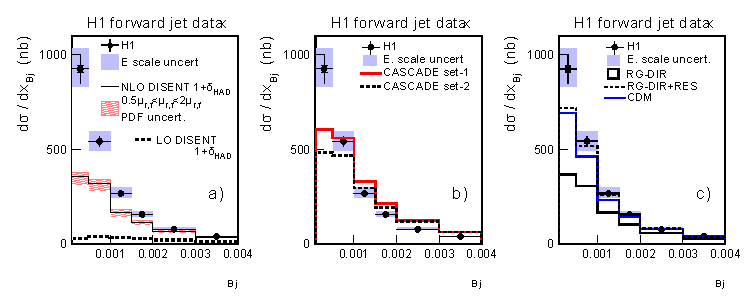
\includegraphics[scale=1]{Afbeeldingen/HERAJets1.eps}
    \caption{Metingen vs Monte-Carlo QCD voorspellingen van inclusieve DIS jetproductie. a) toont dat zeker voor zeer lage $x$, er een grote afwijking is tussen NLO DGLAP en experimentele data. b) toont CASCADE  (een \textit{Monte-Carlo event generator}, gebaseerd op CCFM). c) toont DGLAP (RG+DIR), DGLAP met een geresolveerd foton (RG+DIR+RES, hieronder beschreven) en CCFM/BFKL (CDM). \cite{Kiesling}}
   \label{fig:HERAJets1}
  \end{center}
\end{figure}
DGLAP heeft een inherente ordening in $\vec{k}_\perp$, wat er voor zorgt dat er een lagere werkzame doorsnede optreedt bij zeer lage $x$ dan wat experimenteel wordt waargenomen.
Meer bepaald, DGLAP beschrijft een situatie die in bepaalde kinematische omstandigheden \cite[sectie 3.2]{Kiesling} sterk onderdrukt is volgens de metingen.
DGLAP in zijn pure vorm leidt dus tot foute resultaten, net door zijn ingebouwde sterke $\vec{k}_\perp$-ordening.
Om dit te verhelpen kan er een modificatie aan DGLAP ingevoerd worden, in de vorm van een \textit{geresolveerd foton}, laat een breking van de $\vec{k}_\perp$-ordening toe, zodat de werkzame bij lage $x$ sterk stijgt.
DGLAP+RES geeft een even goede beschrijving als CCFM/BFKL, maar beiden geven nog te lage werkzame doorsneden (zie figuur \ref{fig:HERAJets1}).
\begin{figure} [H]
  \begin{center}
    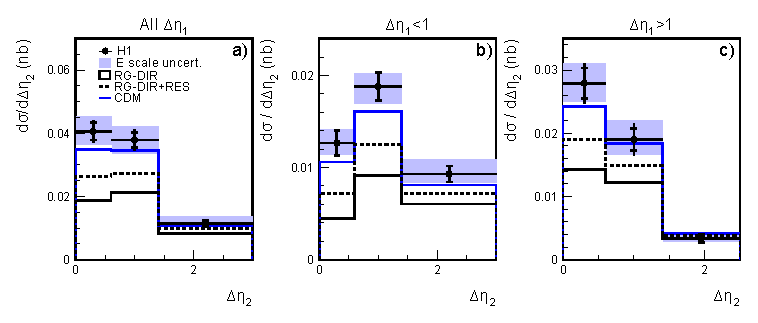
\includegraphics[scale=1]{Afbeeldingen/HERAJets2.eps}
    \caption{Metingen vs Monte-Carlo QCD voorspellingen van DIS dubbele voorwaartse jetproductie. $\eta$ is een \textit{psuedo-rapidity}, gelijk aan $-\ln{\tan{\frac{\theta}{2}}}$. \cite{Kiesling}}
   \label{fig:HERAJets2}
  \end{center}
\end{figure}
Hoewel figuur \ref{fig:HERAJets1} geen onderscheidbaar verschil tussen DGLAP en BFKL toont en dus feitelijk BFKL afschrijft omdat het niet nodig zou zijn om de data goed te beschrijven, geeft figuur \ref{fig:HERAJets2} een andere indruk.
De niet-inclusieve metingen in de tweede figuur geven duidelijk een verschil aan tussen BFKL en DGLAP.
Zelfs met het geresolveerd foton kan DGLAP de data niet goed genoeg beschrijven en geeft BFKL berekeningen doen dit wel.
Dit geeft een duidelijk signaal dat BFKL dynamica wel degelijk optreedt, zij het enkel onder de nodige speciale voorwaarden.
Deze belangrijke waarneming, samen met een natuurlijke saturatie van de structuurfuncties, zoals beschreven wordt in de volgende sectie, geven een sterke motivatie voor het toepassen van BFKL/BK dynamica voor zeer lage $x$ data.
Gebieden met zeer lage $x$ zijn nog maar oppervlakkig gemeten in HERA; de LHeC zal met zijn lager $x$-bereik duidelijkheid kunnen scheppen over waar en hoe de verschillende benadering moeten en kunnen worden gebruikt.

    \subsection{Structuurfuncties}
Een meetbare grootheid die de theorie verbindt met harde waarnemingen, is de structuurfunctie.
Deze waarschijnlijkheidsverdelingen in functie van $x$ en $Q^2$  geven een indicatie van de kans om in een DIS proces met een parton te botsen met die $x$ en $Q^2$.
Met de juiste definities kan men de werkzame doorsnede voor een NC proces (figuur \ref{fig:NC}) als volgt schrijven (als $M^2/Q^2 \rightarrow 0$):
\begin{align} \label{eq:SF}
\frac{d\sigma}{dxdQ^2} &= \frac{2\pi \alpha^2}{xQ^4} \left(Y_+ F_2 \pm Y_- x F_3 - y^2 F_L \right)
\end{align}
Een uitgebreide discussie van bovenstaande uitdrukking staat in appendix \ref{app:SF}.
Als er enkel een foton kan worden uitgewisseld ($\sigma_\gamma \gg \sigma_Z$, dus de interactie via Z wordt verwaarloosd), kan men aantonen dat $F_3 \approx 0$ (zie ook appendix \ref{app:SF}).
In dit werk zal gekeken worden naar het gebied met heel kleine $x$, waardoor saturatie belangrijk wordt.

    \subsubsection{Factorisatie-theorema}
Een handig theorema dat toelaat de perturbatieve en niet-perturbatieve stukken van een  theoretische berekening van elkaar te scheiden.
Voor een DIS interactie ($l+p\rightarrow l’+X$) heeft de volgende vorm \cite{Martin}: 
\begin{equation}
F_a(x, Q^2) = \sum*{i=q,q,g} \int_0^1 \frac{dy}{y} f_i(y, Q^2) C_{a,i} \left( \frac{x}{y},\alpha_S(Q^2) \right) + O \left( \frac{\Lambda_{QCD}^2}{Q^2} \right) 
\end{equation}
$F_a$ is een structuurfunctie.
$f_i$ is een universele partondichtheid die geldig is onder alle omstandigheden.
Deze kan niet perturbatief worden uitgerekend, maar met behulp van DGLAP kan hun $Q^2$ afhankelijkheid bepaald worden.
$C_{a,i}$ zijn coëfficiëntfuncties, die een subproces op korte afstand beschrijven.
Deze kan men wel perturbatief uitrekenen, maar verschillen naar gelang het beschouwde proces.
Deze algemene vorm wordt vaak gebruikt en is geldig tot alle ordes in perturbatietheorie.
De keuze van de factorisatie zelf (welk deel waar in gestopt wordt) staat nog vrij en kan later berekeningen vereenvoudigen.
Het is duidelijk dat de resultaten onafhankelijk moeten zijn van het factorisatieschema (dat vaak gepaard gaat met de invoering van een nieuwe schaalvariabele).

    \subsubsection{Saturatie} \label{sec:Saturatie}
Saturatie zal in een of andere vorm moeten optreden voor zeer kleine $x$, omdat anders de partondichtheden (in het bijzonder, maar niet enkel die van het gluon) niet fysisch meer zijn en de huidige formulering onzinnige resultaten zou voorspellen (zie figuur \ref{fig:PD}).
In dit werk wordt dus uitbundig gebruik gemaakt van modellen die met dit fenomeen rekening houden.

      \paragraph{GBW-model}
Een beproefd en op zich eenvoudig model, is dat van Krzysztof Golec-Biernat \cite{GB}.
Golec-Biernat gebruikt het formalisme van de foton golffunctie (een vorm van het factorisatie theorema), waarbij een foton onafhankelijk van de DIS botsing kan splitsen in een $q\bar{q}$-paar, dat dan interageert met het proton.
Dit laat toe een perturbatieve berekening te doen voor deze golffunctie, en de rest wordt beschreven door middel van een model.
\begin{align}
\sigma_{T,L} = \int d^2 \vec{r} \int_0^1 dz |\Psi_{T,L} (z, \vec{r})|^2 \hat{\sigma} (x,r^2)
\end{align}
Waarbij $\Psi$ de golffunctie van het foton is, $T$ en $L$ duiden op respectievelijk het longitudinaal en het transversaal deel hiervan, en $\hat{\sigma}$ het gemodelleerde, niet-perturbatieve gedeelte is.
Bovenstaande vergelijking is geformuleerd in positieruimte.
$r$ is de afstand tussen het ontstane $q\bar{q}$-paar.
Golec-Biernat en Wüsthoff bespreken in \cite{GBW} wat het GBW model wordt genoemd.
Dit model kan in impulsruimte en in positieruimte gebruikt worden.
De saturatie zit in de factor $\hat{\sigma}$, die de volgende vorm heeft:
\begin{align}
\hat{\sigma}(x,r^2) &= \sigma_0 \left[ 1- \exp{\left(-\frac{r^2}{4 R_0^2(x)}\right)} \right] \\
R_0^2(x) &= \frac{1}{Q_0^2} \left( \frac{x}{x_0} \right)^\lambda \label{eq:R0}
\end{align}
\eqref{eq:R0} is de \textit{saturation radius}, wat effectief een saturatie schaal invoert voor $r$.
$Q_0^2$ is 1 GeV, en ingevoerd om de juiste dimensies te krijgen.
$\sigma_0$, $\lambda$ en $x_0$ zijn de parameters van het model, die bepaald zijn door te fitten aan alle DIS data die beschikbaar was.
Ze verschillen voor het geval waar enkel $uds$ quarks bijdragen en waar ook de charm quark bijdraagt (zie appendix \ref{app:GBWParameters}).
Dit model heeft een ingebouwde begrenzing van de dipool werkzame doorsnede $\hat{\sigma}$.
Deze heeft het juiste gedrag in $r$: kwadratisch voor kleine $r$, en constant voor grote waarden.
Dat $\hat{\sigma}$ nul is voor kleine dipoolstraal $r$, hoeft geen verwondering.
Als de afstand $r$ tussen de twee quarks van $q\bar{q}$-paar klein is, zal het vanop redelijke afstand een kleurneutraal object vormen en kan er dus geen QCD interactie optreden.
Dit effect heet kleurdoorzichtigheid.
Een ander sterk punt van dit model is het feit dat hier een saturatie voor kleine $x$ is ingebouwd, wat natuurlijk wenselijk is voor berekeningen in dat gebied.

      \paragraph{Zware quarks}
GBW hebben ook in \cite{GBW} aangetoond dat het beschouwen van een extra (zware) quark, namelijk de charm, leidt tot een saturatie-effect.
Het bestuderen van de structuurfuncties in het licht van dit effect is zeer interessant, en wordt dieper op ingegaan in sectie \ref{sec:SF} en \ref{sec:ResSF}.

  \subsection{Dwarse energiestroom}
    \subsubsection{Belang van de LHeC}
Om met zekerheid te kunnen spreken over de resultaten van deze berekeningen en een definitieve grens te kunnen trekken tussen DGLAP en BFKL qua geldigheidsgebieden.
Hiernaast zal de uitbreiding van het kinematische gebied waarin metingen kunnen worden gedaan ertoe bijdragen dat een groter deel van \textit{the Big Picture} zichtbaar wordt, waardoor de drie verschillende aanpakken van nu eventueel kunnen veralgemeend worden naar iets dat in zichzelf op z’n minst een breder toepassingsgebied heeft.
HERA was de vorige elektron-proton versneller, en heeft de deur opengezet naar een hele reeks belangrijke metingen in daarvoor onbereikbare gebieden.
Een massamiddelpuntsenergie van 318 GeV maakte het mogelijk om onder andere DIS  interacties te onderzoeken met $x$ zo klein als $10^-4$ en $Q^2$ zo groot als $10^3$ GeV.
Aan die ondergrens voor $x$ toonde HERA ook een aanzet tot nieuwe fysica, die door de huidige theorie onvoldoende wordt voorspeld (zie sectie \ref{sec:QCDvsExperiment} voor een uitgebreide discussie hierover).
Een aanzet die vervolledigd kan worden door het zeer lage $x$-regime verder te onderzoeken.
Hiervoor is een krachtigere versneller dan HERA nodig, zoals het huidige LHC.
Deze laatste produceerd botsingen tussen protonen, met een massamiddelpuntsenergie van rond en boven de 14 TeV.
Het grote probleem met de LHC en DIS botsingen, is de contaminatie van de geproduceerde deeltjes.
Twee protonen die tegen zo’n hoge snelheden met elkaar botsen, zorgen voor enorm veel ruis in de vorm van extra deeltjes als men de pure DIS interactie wil onderzoeken.
Als men het proton door een elektron vervangt (dat niet uit quarks en gluonen bestaat), gaat er ongeveer de helft minder hadronisatie optreden zodat er een zuiverder signaal uit de detector komt.
Als men met versnelde elektronen werkt, moet men natuurlijk ervoor uitkijken dat de synchrotronstraling de versnelling niet tenietdoet.
Synchrotronstraling is energie uitgestraald door een elektron als het in een cirkelvormige baan versneld wordt.
Het kost dus nóg meer energie om elektronen boven die grens van synchrotronstraling te krijgen zonder te veel verlies aan snelheid.

    \subsubsection{Waarom kijken naar $E_T$ met BFKL dynamica}
De transversale energiestroom is misschien wel de interessantste grootheid om de eigenschappen van DIS interacties te bestuderen.
Bij een botsing tussen protonen botsen, komen er ook deeltjes vrij die een niet-collineaire impuls hebben.
In tegenstelling tot de protonen die collineair botsen en dus geen $\vec{k}_\perp$ hebben, kunnen de partonen in het proton wel een transversale impuls hebben.
De transversale energiestroom is dus voor een groot deel afkomstig uit een interactie met een parton dat in tegenstelling tot het proton, een transversale impuls heeft.
Dit is dan ook de reden dat de transversale energiestroom, in tegenstelling tot de uitgaande protonresten, een goede bron van informatie is over harde parton-parton interacties.

    \subsubsection{Formulering van $E_T$}
\begin{figure} [H]
  \begin{center}
    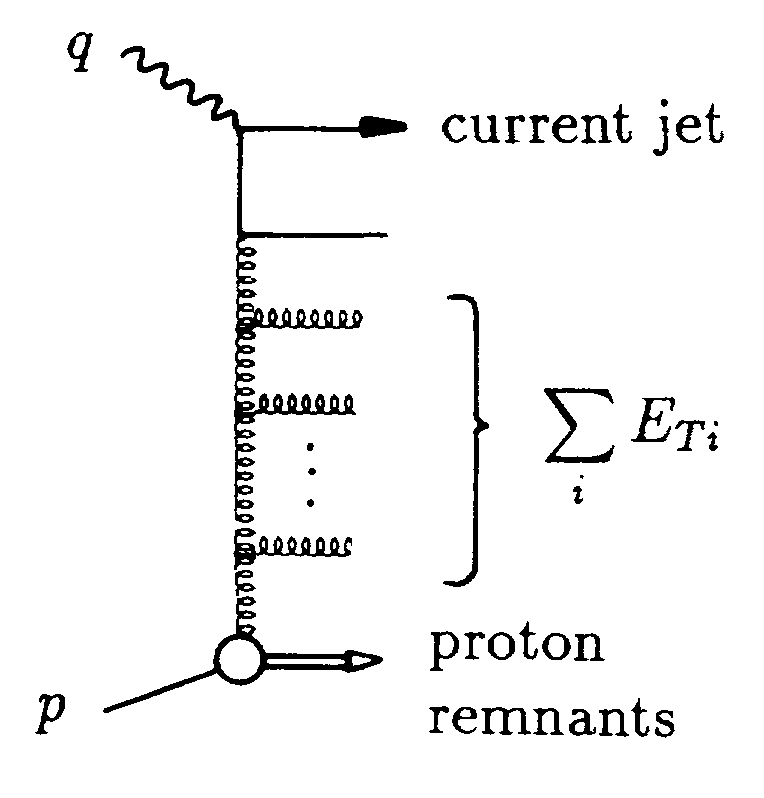
\includegraphics[width=.33\textwidth]{Afbeeldingen/ETDefinitionDiagram.png}
    \caption{DIS interactie met de totale $E_T$ aangeduid. \cite{ET}}
   \label{fig:ETDefinitionDiagram}
  \end{center}
\end{figure}
In \cite{ET} wordt een uitdrukking berekend voor de transversale energiestroom van een DIS botsing.
In figuur \ref{fig:ETDefinitionDiagram} wordt duidelijk aangeduid welke emissies bij $E_T$ worden gerekend.
Golec-Biernat, Kwieciński, Martin en Sutton zijn vertrokken van het diagram weergegeven in figuur \ref{fig:ETDiagram}.
\begin{figure} [H]
  \begin{center}
    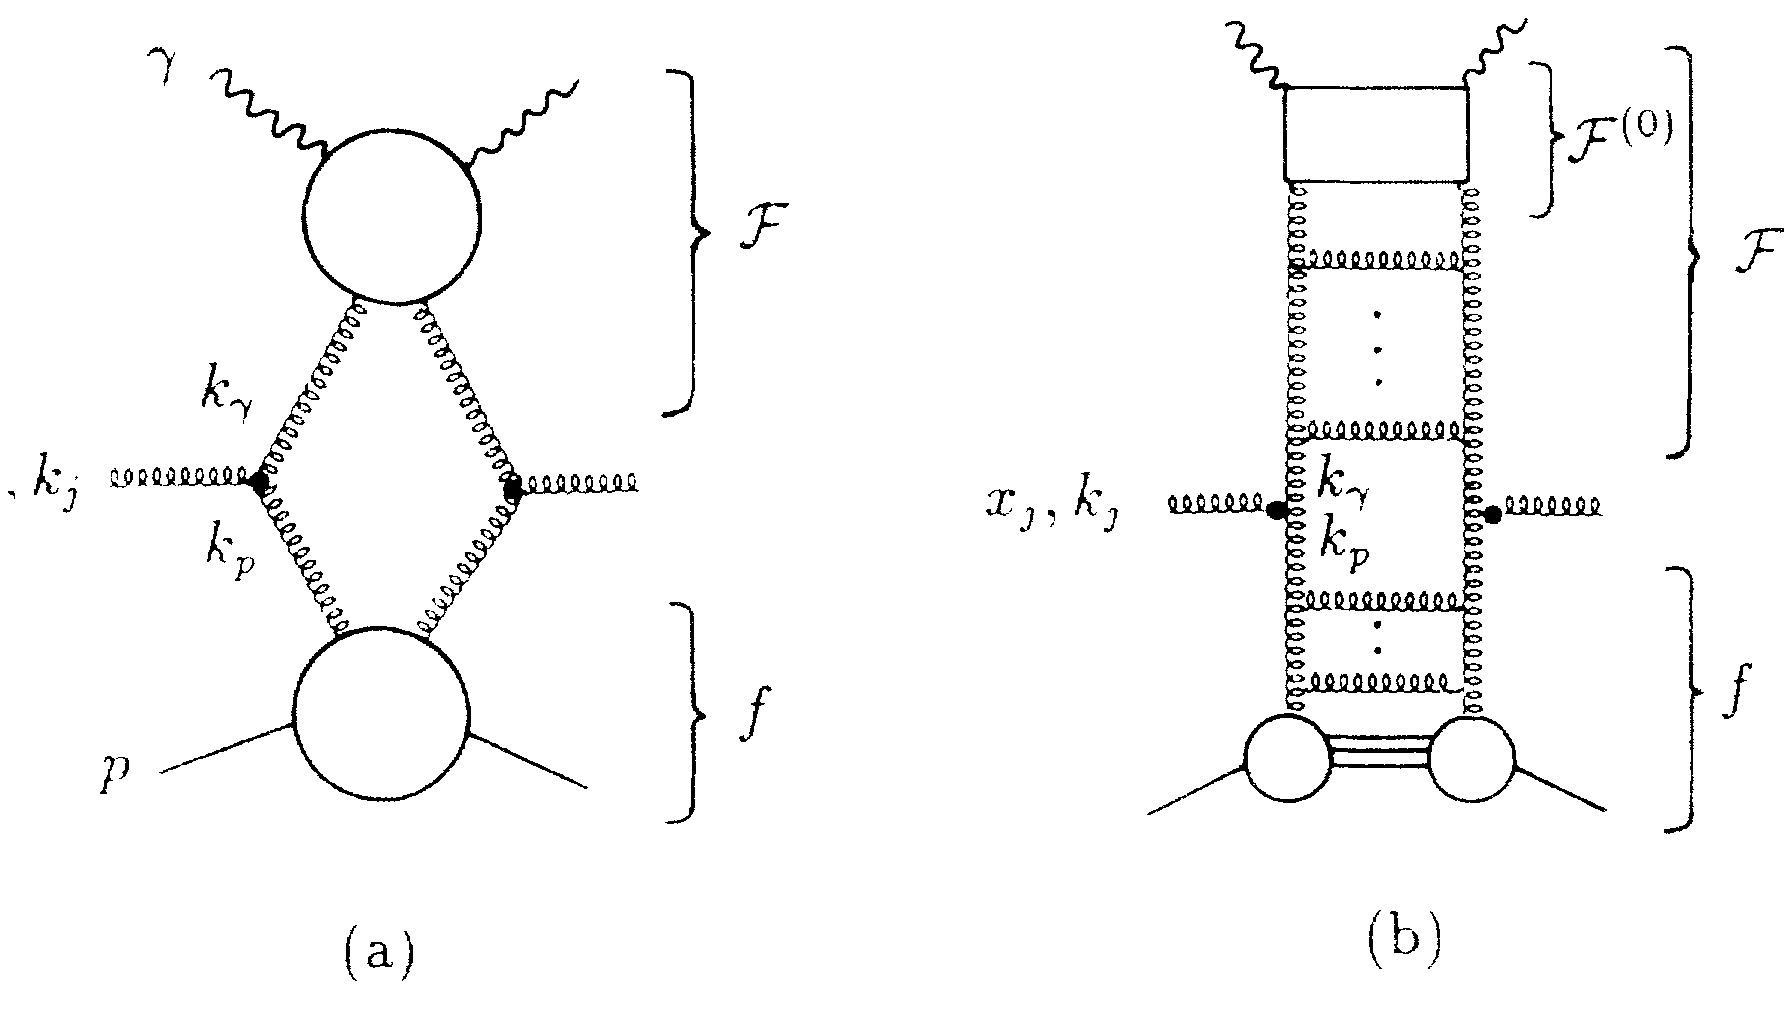
\includegraphics[width=.66\textwidth]{Afbeeldingen/ETDiagram.png}
    \caption{a) illustreert formule \eqref{eq:ETGluonChain}. b) toont expliciet de door BFKL gehersommeerde gluonladders. \cite{ET}}
   \label{fig:ETDiagram}
  \end{center}
\end{figure}
De transversale energiestroom van een gluonladder zoals weergegeven in figuur \ref{fig:ETDiagram} (a) (en expliciet getoond in (b) ), heeft de volgende vorm:
\begin{equation} \label{eq:ETGluonChain}
x_j \frac{\partial E_T}{\partial x_j} = \frac{1}{\sigma} \int dk_j^2 x_j \frac{\partial \sigma}{\partial x_j \partial k_j^2} |\vec{k}_j|
\end{equation}
$x_j$  en $\vec{k}_j$ zijn respectievelijk de longitudinale impulsfractie en de transversale impuls van de gluon jet in het proton-proton massamiddelpuntstelsel.
De differentiële werkzame doorsnede kan uitgedrukt worden in functie van de structuurfuncties van het proton.
\begin{equation}
\frac{\partial \sigma}{\partial x_j \partial k_j^2} = \frac{4 \pi \alpha^2}{xQ^2} \left[ (1-y) \frac{\partial F_2}{\partial x_j \partial k_j^2} + \frac{1}{2} y^2 \frac{\partial 2xF_1}{\partial x_j \partial k_j^2} \right]
\end{equation}
Waarbij $y=Q^2/xs$ en $\sqrt{s}$ gelijk aan de massamiddelpuntsenergie van het elektron-proton systeem.
Deze uitdrukking werden uitgerekend voor kleine $x$ (dus met behulp van BFKL dynamica), en ingevuld met vergelijkingen die toen de beste resultaten gaven.
Hier zal vergelijking  \eqref{eq:ET} opnieuw beschouwd worden, en toegepast op hernieuwde uitdrukkingen voor de samenstellende formules.
\begin{align} \label{eq:ET}
x_j \frac{\partial E_T}{\partial x_j} = \frac{1}{F_2} \int \frac{dk_p^2}{k_p^2} \int \frac{dk_\gamma^2}{k_\gamma^2} \left( \frac{3\alpha_S}{\pi} \right) \mathcal{F}_2 \left( \frac{x}{x_j}, k_\gamma^2, Q^2 \right) f(x_j,k_p^2) \int \frac{d\phi}{\sqrt{k_p^2+k_\gamma^2 + 2k_p k_\gamma \cos{\phi}}}
\end{align}
Deze uitdrukking bestaat uit verschillende, afzonderlijk te beschouwen delen, die elk op hun beurt even interessant zijn.
$F_2 (x, Q^2)$ is de structuurfunctie van het proton, $f$ is de ongeïntegreerde gluondichtheid van het proton en $\mathcal{F}_2$ is de structuurfunctie van de hadronische structuur van het foton.
Belangrijk op te merken is dat $F_2$ op voorhand kan berekend worden, en de integraal over $\phi$ analytisch kan worden bepaald.
 
    \subsubsection{Ongeïntegreerde gluondichtheid van het proton $f$}
Golec-Biernat en Wüsthoff hebben deze grootheid in het kader van hun model berekend, en heeft volgende uitdrukking \cite[vgl. 9.255]{Barone}:
\begin{equation}
f(x,k^2) = \frac{3 \sigma_0}{4\pi^2 \alpha_S} R_0^2 (x) k^4 e^{-R_0^2(x) k^2}
\end{equation}
Waarbij
\begin{equation}
R_0^2(x) = \frac{1}{Q_0^2} \left( \frac{x}{x_0} \right)^\lambda
\end{equation}
De gebruikte parameters staan vermeld in appendix \ref{app:GBWParameters}.
het diagram in \ref{fig:ETDiagram} (b) toont $f$.
Dit is ook een ingrediënt voor de formule voor de volgende sectie.

    \subsubsection{$F_2$} \label{sec:SF}
De structuurfunctie $F_2 = F_L + 2x F_1$ is te vinden in \cite[vgl. 9.200]{Barone} en kan als volgt worden geschreven:
\begin{align} \label{eq:MasslessSF}
F_2(x,Q^2) &= \frac{Q^2}{4\pi^2} \alpha_S \sum_q e_q^2 \int_0^\infty \frac{dk}{k^2}\pi f(x,k^2) \int_0^1 d\rho \int_0^1 d\eta \times \Phi_2(\rho, \eta, Q^2, k^2) \\
\text{met } \Phi_2(\rho, \eta, Q^2, k^2) &= \frac{1-2\rho(1-\rho)-2\eta(1-\eta)+12\rho(1-\rho)\eta(1-\eta)}{Q^2 \rho(1-\rho) + k^2 (\eta(1-\eta)}\notag \\
F_L(x,Q^2) &= \frac{2 Q^2}{\pi^2} \alpha_S \sum_q e_q^2 \int_0^\infty \frac{dk^2}{k^2} \pi f(x,k^2) \times \Phi_L(\rho, \eta, Q^2, k^2) \\
\text{met } \Phi_L(\rho, \eta, Q^2, k^2) &= \frac{\rho(1-\rho)\eta(1-\eta)}{Q^2 \rho(1-\rho)+k^2 \eta(1-\eta)} \notag
\end{align}
$e_q$ is de lading van de quark en de som loopt over de beschouwde quarks.
De functie $f$ is gedefinieerd in de vorige sectie.
\eqref{eq:MasslessSF} is bedoeld voor gebruik met de 3 quark parameters in appendix \ref{app:GBWParameters}.
In \cite{Bondarenko} wordt een formule voor $F_2$ gepresenteerd die uit de BK vergelijking werd afgeleid.
Deze houdt rekening met 4 quarks en dus hun afzonderlijke massa.
De exacte formule voor $F_2$ wordt niet weergegeven, maar de longitudinale en transversale delen wel.
De relatie tussen de verschillende structuurfuncties wordt weergegeven in appendix \ref{app:SF}.
\begin{align} \label{eq:MassiveSF}
&\Phi_L(k^2, m_q^2) \sim \sum_q e_q^2 \int_0^1 d\rho \int_0^1 d\eta \frac{k^2 \eta(1-\eta)\rho^2(1-\rho)^2 Q^2}{(Q^2\rho(1-\rho)+k^2\eta(1-\eta)+m_q^2)(Q^2\rho(1-\rho)+m_q^2)} \\
&\Phi_T(k^2, m_q^^2) \sim \sum_q e_q^2 \int_0^1 d\rho \int_0^1 \eta \notag \\
&\frac{k^2 Q^2 (\rho^2+(1-\rho)^2)\rho(1-\rho)(\eta^2+(1-\eta)^2)+k^2(\rho^2+(1-\rho)^2)m_q^2 + 4\rho(1-\rho)\eta(1-\eta)m_q^2}{(Q^2\rho(1-\rho)+k^2\eta(1-\eta)+m_q^2)(Q^2\rho(1-\rho)+m_q^2)}
\end{align}
$m_q^2$ is de massa van de afzonderlijke quarks, zoals weergegeven in appendix \ref{app:GBWParameters}.

    \subsubsection{$\mathcal{F}_2$} \label{sec:UGD}
De structuurfunctie van de hadronische structuur van het foton is een exotische grootheid waar nog veel onduidelijkheid over bestaat.
Het wordt ook wel eens aangeduid als \textit{ongeïntegreerde gluondichtheid in het foton}.
Hier wordt gebruik gemaakt van een berekening waar een initïele toestand $\mathcal{F}^{(0}$ werd geëvolueerd met behulp van de BK vergelijking [CITATION NEEDED].
Figuur \ref{fig:ETDiagram} (b) toont de begintoestand, namelijk de \textit{quark doos}, die werd aangenomen als beginvoorwaarde bij het oplossen van de BK vergelijking.
Voor de volledigheid worden hier de formule met en zonder evolutie gegeven.
De resultaten worden getoond in sectie \ref{sec:ResUGD}.
\begin{align} \label{eq:UGD}
\mathcal{F}_\text{zonder evolutie} &= TODO \\
\mathcal{F}_\text{met evolutie} &= TODO
\end{align}

\section{Numerieke aanpak}
Om de berekeningen zelf zo vlot mogelijk te laten verlopen, werd gekozen voor een implementatie in C++.
Alle afzonderlijke formules werden gecontroleerd door vergelijking met een implementatie in Mathematica 7, door de auteur zelf en door Krzysztof Kutak.

  \subsection{Numerieke integraties}
Omdat in alle formules afzonderlijk ten hoogste drie numerieke integraties tegelijk aan te pas komen, werd gekozen om Monte-Carlo integratie te vermijden.
Steve G. Johnson heeft een implementatie in C geschreven voor het numeriek integreren in een willekeurig aantal dimensies van een willekeurige functie (mogelijk ook multidimensionaal).
De beschrijving van het algoritme zelf staat uitvoerig beschreven in \cite{Genz} en \cite{Berntsen}.
Hoewel het algoritme gebaseerd is op de kubatuur regels, is het een adaptief en efficiënt algoritme voor multi-dimensionale integraties.
Het vertoonde geen fundamentele problemen met de afzonderlijke formules uit sectie \ref{sec:SF} en \ref{sec:UGD}, hoewel deze vol singulariteiten zitten en problematisch kunnen zijn.

  \subsubsection{Berekening van$E_T$}
De uiteindelijke formule bestaat uit vier delen:
\begin{itemize}
  \item $F_2$, die per waarde een enkele keer moet worden berekend.
  \item $f$, waarover wordt geïntegreerd, bevat geen verborgen integraties en hoeft dus geen speciale behandeling.
  \item $\mathcal{F}_2$, die zelf drie integraties bevat, wordt per waarde van $x$ en $Q^2$ geïnterpoleerd in het nodige interval van de variabele $x$, om zo de berekening een stuk sneller te laten verlopen,
  \item de integraal in $\phi$, die analytisch uitgerekend kan worden (zie appendix \ref{app:PhiIntegral}), maar als integraal behouden is wegens redenen vermeld in appendix \ref{app:PhiIntegral}.
\end{itemize}

Interpolatie werd geïmplementeerd met behulp van de GNU Scientific Library (GSL), die een handige en snelle oplossing voor een ééndimensionale interpolatie biedt.
De uiteindelijke driedimensionale integraal kon niet in een redelijke tijd worden uitgerekend door het \textit{Cubature} algoritme, dus werd voor de laatste stap gekozen voor Monte-Carlo integratie, wederom die van GSL.
De resultaten van de uiteindelijke berekening zijn dan ook minder accuraat, omdat enerzijds de Monte-Carlo integratie vrij veel tijd in beslag nam en anderzijds de fout vrij hoog en wisselend bleef bij hoge aantallen van iteraties.

\section{Resultaten}
    \subsection{De structuurfuncties van dichtbij bekeken} \label{sec:ResSF}
$F_2$ en $F_L$ zijn interessante grootheden, zeker in het licht van saturatie en de B(F)K(L) vergelijking.
Door vergelijkingen \eqref{eq:MasslessSF} (en bijhorende formule voor $F_L$ \cite[sectie 9.5.4]{Barone}) en \eqref{eq:MassiveSF} uit te rekenen, kan men zien dat $F_2$ nagenoeg niet verandert door invoering van de extra quark (en dus saturatie), maar $F_L$ is er wel onderhevig aan.
In figuur \ref{fig:ResSF} staan de resultaten van de formules \eqref{eq:MasslessSF} en \eqref{eq:MassiveSF} uitgezet, samen met data van HERA \cite{H1} \cite{ZEUS} indien beschikbaar.
De derde curve op de grafiek werd berekend in \cite{Stasto} en verschilt in aanpak en benadering van de berekening hier.
Enerzijds houdt de derde curve geen rekening met saturatie en toont dus de invloed van het fenomeen in het GBW model.
De berekening gebruikt een geünificeerde DGLAP-BFKL aanpak, die overeen komt met een lineaire evolutievergelijking.
De formules \eqref{eq:MassiveSF} en \eqref{eq:MassiveSF} stammen voort uit een tweede orde correctie daarop (die dus met saturatie rekening houdt) en stamt uit een niet-lineaire evolutievergelijking (BK).
Anderzijds wordt daar wel gewerkt met exacte kinematica, wat wil zeggen dat in plaats van de simpele veronderstelling $x_g=x_{Bj}$ die hier gemaakt wordt, er een ingewikkeldere relatie toegepast wordt.
Dit brengt hogere orde correctietermen met zich mee, die niet in \eqref{eq:MassiveSF} en \eqref{eq:MassiveSF} zitten.
\begin{figure} [H]
  \begin{center}
    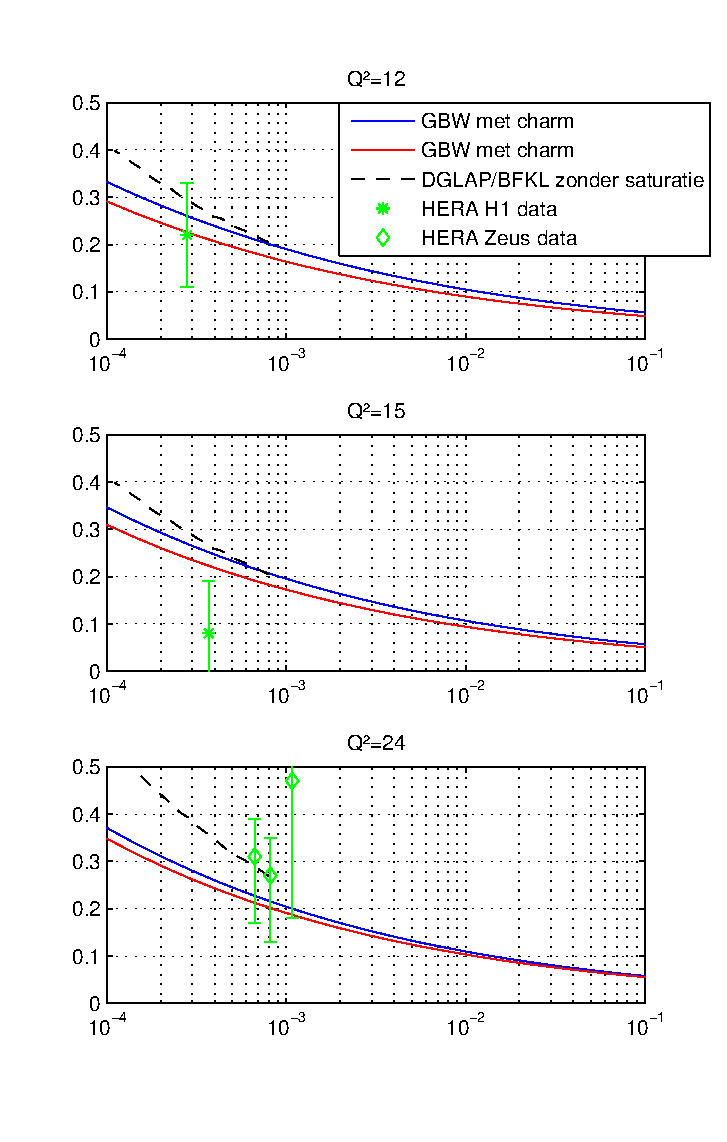
\includegraphics[width=.75\textwidth]{Afbeeldingen/PlotFL.eps}
    \caption{Plot van $F_L$ voor verschillende waarden van $Q^2$ in functie van $x$.}
   \label{fig:ResSF}
  \end{center}
\end{figure}
Het is duidelijk dat bij GBW saturatie de structuurfunctie kleiner is dan zonder, dit is natuurlijk het gewenste effect.
Niet getoond, maar wel belagrijk te vermelden is het feit dat de gebruikte berekeningen niet goed opgaan voor hogere waarden van $Q^2$, waardoor meer plots (voor bijvoorbeeld ZEUS’ $Q^2=60, 80, 110$) geen goede resultaten geven.

  \subsection{De ongeïntegreerde gluondichtheid van het foton} \label{sec:ResUGD}
De ongïntegreerde gluondichtheid is tot nu toe enkel gemodelleerd als bijdrage aan een proces, en nooit afzonderlijk gemeten.
Hier wordt de gluondichtheid ook ingevoerd om een \textit{geresolveerd foton} te krijgen (gelijkend op de correcties op DGLAP in figuren \ref{fig:HERAJets1} en \ref{fig:HERAJets2}).
Een belangrijk verschil met het geresolveerd foton in een DGLAP berekening zoals getoond in \cite{Kiesling}, is dat hier een BFKL berekening word toegepast die op een natuurlijke wijze saturatie omvat door zwaardere quarks zoals beschreven in het GBW model.
De resultaten worden weergegeven in figuur \ref{fig:ResUGD}.
\begin{figure} [H]
  \begin{center}
    \includegraphics[scale=1]{Afbeeldingen/Placeholder.eps}
    \caption{Plot van $\mathcal{F}_2$ zoals gebruikt in de berekening van $E_T$.}
   \label{fig:ResUGD}
  \end{center}
\end{figure}

  \subsection{De transversale energiestroom} \label{sec:ResET}
De transversale energiestroom in een DIS interactie is berekend met behulp van \eqref{eq:ET} en bijhorende subformules.
De resultaten worden weergegeven in figuur \ref{fig:ResET}.
\begin{figure} [H]
  \begin{center}
    \includegraphics[scale=1]{Afbeeldingen/Placeholder.eps}
    \caption{Plot van $F_L$ voor verschillende waarden van $Q^2$ in functie van $x$.}
   \label{fig:ResET}
  \end{center}
\end{figure}

\section{Bespreking}



\section{Besluit}



\newpage
\appendix
\section{Diep Inelastische Verstrooiing} \label{app:DIS}
Als men figuur \ref{fig:DIS} beschouwt in het IMF ($m_e \approx m_p \approx 0$), geldt wegens behoud van energie:
\begin{align}
&(xP+q)^2 = m_e = 0 \notag \\
\Leftrightarrow &x^2 P^2 + 2xPq + q^2 = 0 \notag \\
\Leftrightarrow &2xPq -Q^2=0
\end{align}
Waarbij gebruikt is dat $-q^2 = Q^2 \gg x^2P^2$ in het  IMF. Dit laatste is equivalent met \eqref{eq:Bjorkenx}.

\section{DIS werkzame doorsnede} \label{app:SF}
Uit kwantum veldentheorie kan men de werkzame doorsnede voor een NC proces zoals in figuur \ref{fig:NC} halen:
\begin{align}
\frac{d\sigma}{dxdQ^2} &= xs \frac{d\sigma}{dxdQ^2} = \frac{2\pi y \alpha^2}{Q^4} \sum_j \eta_j L_j^{\mu \nu} W_{\mu \nu}^j
\end{align}
Waarbij de som over j loopt over
\begin{itemize}
  \item $\gamma$, met $\eta_\gamma=1$,
  \item $\gamma Z$, met $\eta_{\gamma Z} = \left( \frac{G_F M_Z^2}{2\sqrt{2}\pi \alpha} \right) \left(\frac{Q^2}{Q^2+M_Z^2} \right)$,
  \item $Z$, met $\eta_Z = \eta_{\gamma Z}^2$.
\end{itemize}
Hier stelt de tweede term de foton en Z uitwisseling voor, en de interferentie tussen de twee. $G_F$ is de Fermi koppeling en $\alpha$ de QED koppeling.
Er is naast $x$ en $Q^2$ nog een derde variabele nodig, die te maken heeft met de totale energie van het systeem.
Dit kan de Mandelstam variabele s zijn, of het relatieve energieverlies van het elektron in het massamiddelpuntsysteem y, zoals hieronder gedefinieerd.
\begin{align}
y &= \frac{p \cdot q}{p \cdot k} = \frac{\Delta E}{E} ,& s = (k+p)^2 \simeq \frac{Q^2}{xy}
\end{align}
$y$ is een Lorentz invariante parameter voor de verstrooiingshoek $\hat{\theta}$ in het massamiddelpuntstelsel.
In dit geval geldt volgende relatie:
\begin{align}
y = \frac{1}{2} \left( 1-\cos{\hat{\theta}} \right)
\end{align}
$L^{\mu \nu}$ is de gekende tensor van het lepton knooppunt in functie van $k$ en $k'$.
$W_{\mu \nu}$ is een onbekende tensor van het hadron knooppunt.
Deze laatste kan dus enkel geparametriseerd worden aan de hand van wat wel gekend is.
De algemene uitdrukking in het geval van niet gepolariseerde DIS is als volgt:
\begin{equation}
W_{\mu \nu} = \left( -g_{\mu \nu} + \frac{q_\mu q_\nu}{q^2} \right) F_1(x,Q^2) + \frac{\hat{P}_\mu \hat{P}_\nu}{p \cdot q} F_2(x,Q^2) -  i\epsilon_{\mu \nu \alpha \beta} \frac{q^\alpha p^\beta}{2p \cdot q} F_3(x,Q^2)
\end{equation}
Hier zijn $F_i$ de structuurfuncties, afhankelijk van $x$ en $Q^2$.
De derde term bevat een uitwendig product (de $\vec{q} \times \vec{q}$ vorm), waardoor deze term pariteit niet behoudt.
Deze term zal dan ook $\approx 0$ indien de Z bijdrage verwaarloosbaar is, omdat voor zover gekend pariteit nog steeds behouden is voor de sterke wisselwerking.
Men bekomt \eqref{eq:SF} door $L^{\mu \nu}$ in te vullen en volgende variabelen te definiëren:
\begin{align}
Y_\pm &= 1 \pm (1-y)^2 \notag \\
F_L &= F_2 - 2x F_1 \notag
\end{align}
In DIS processen, kan men vaak uitgaan van $F_L = 0$, zodat $F_2$ in dat geval voldoende is om de hele werkzame doorsnede te bepalen.
De longitudinale en transversale structuurfuncties hebben het volgende verband met $F_2$ en $F_1$:
\begin{align}
F_2 &= F_L + F_T \\
F_2 &= F_2 - 2xF_1 \notag
\end{align}

\section{Renormalisatiegroep vergelijking en asymptotische vrijheid} \label{app:RGE}
Het tweede deel van vergelijking \eqref{eq:RGE} wordt als volgt bekomen \cite{Ellis}.
Vertrekkende van het stuk voor de dubbele pijl, en volgende nieuwe variabele $t$ en functie $\beta$:
\begin{equation}
t = \ln{\frac{Q^2}{\mu^2}}, \beta(\alpha_S) =  \frac{\partial \alpha_S}{\partial \ln{\mu^2}}
\end{equation}
Waarbij de partiële afgeleide genomen wordt in $\alpha_S$ = de kale koppelingsconstante.
Vergelijking \eqref{eq:RGE} kan nu herschreven worden:
\begin{equation}
\left[ -\frac{\partial}{\partial t} + \beta(\alpha_S) \frac{\partial}{\partial \alpha_S} \right] R(e^t, \alpha_S) = 0
\end{equation}
Deze vergelijking kan men oplossen door een nieuwe functie te definiëren, namelijk de lopende koppeling $\alpha_S(Q^2)$, waarvoor het volgende moet gelden:
\begin{equation} \label{eq:AlphaSDefinition}
t = \int_{\alpha_S}^{\alpha_S(Q^2)} \frac{dx}{\beta(x)}, \alpha_S(\mu^2) := \alpha_S
\end{equation}
Door de voorgaande vergelijking te differentiëren, kan men schrijven:
\begin{align}
\frac{\partial \alpha_S(Q^2)}{\partial t} &= \beta( \alpha_S(Q^2) ) \notag \\ \frac{\partial \alpha_S(Q^2)}{\partial \alpha_S} &= \frac{\beta(\alpha_S(Q^2))}{\beta(\alpha_S)}
\end{align}
Waaruit de enkele $\alpha_S(Q^2)$-afhankelijkheid volgt.
Een observabele is afhankelijk van de schaalvariabele, maar deze afhankelijkheid komt tot uiting door de afhankelijkheid van de observabele van $\alpha_S$.
Men kan dus een observabele uitrekenen voor een vaste waarde van $\alpha_S$, en met behulp van vergelijking \eqref{eq:AlphaSDefinition} variëren met $Q^2$.

\section{Parameters van het GBW model voor saturatie} \label{app:GBWParameters}
In het geval van 3 lichte quarks: up, down en strange, krijgt men volgende waarden:
\begin{align}
\sigma_0 &= 23,03 \text{mb} \notag \\
\lambda &= 0,288 \\
x_0 &= 3,04 \times 10^{-4} \notag
\end{align}
In geval van een vierde charm quark zijn de gefitte waarden anders.
\begin{align}
\sigma_0 &= 29,12 \text{mb} \notag \\
\lambda &= 0,277 \\
x_0 &= 0,41 \times 10^{-4} \notag
\end{align}
De waarden komen overeen met die in \cite{GBW}.
De massa’s van de quarks waarvoor deze parameters werden bepaald zijn de volgende:
\begin{align}
m_u &= m_d = m_s = 0,14 \text{GeV}\notag \\
m_c &= 1.5 \text{GeV}
\end{align}
Een andere waarde voor deze massa’s en/of de introductie van een vijfde quark ($b$) zonder bovenstaande parameters opnieuw te bepalen is onjuist.

\section{De ordening in hoeken in CCFM} \label{app:CCFM}
Om \eqref{eq:HoekOrdening} uit te drukken in impulsfracties, heeft men volgende definities nodig:
\begin{align}
\theta_i = \frac{q_i}{(1-z_i)E_{i-1}}, z_i = \frac{E_i}{E_{i-1}}
\end{align}
Waarbij $q_i$, $\theta_i$ en $E_i$ respectievelijk de transversale impuls, uitstralingshoek en energie zijn van het $i$-de gluon.
Nu kan men
\begin{equation}
\theta_{i+1} > \theta_i
\end{equation}
 vervangen door:
\begin{equation}
 \frac{q_{i+1}}{1-z_{i+1}} > \frac{z_i q_i}{1-z_i}
\end{equation}
Wat voor $z_i, z_{i+1} \ll 1$ reduceert tot $q_{i+1} > z_i q_i$.
Belangrijk op te merken is dat in de hoge energie limiet, CCFM dezelfde oplossing oplevert als de BFKL vergelijking.
Voor verdere discussie geeft \cite{Vera} een goed overzicht van CCFM en de verhouding hiervan met BFKL.

\section{Integraal over $\phi$} \label{app:PhiIntegral}
De integraal over $\phi$ in \eqref{eq:ET} kan analytisch worden uitgerekend.
Mathematica geeft als analytisch resultaat voor een integraal van de volgende vorm:
\begin{equation}
\int_0^{2\pi} \frac{1}{\sqrt{a + b \cos{\Phi}}}
\end{equation}
Volgende oplossing:
\begin{equation}
\frac{2 \sqrt{a + b} K(-\frac{2b}{a - b}) + \sqrt{a - b} K(\frac{2b}{a + b})}{\sqrt{a^2 - b^2}}
\end{equation}
Waarbij $K$ de volledige elliptische integraal van de eerste soort is zoals gedefinieerd op Wolfram Alpha onder “EllipticK”.
Het probleem met deze analytische oplossing is dat alle gevonden implementaties in C of C++ van de elliptische integraal, het domein van het argument beperken tot $[0,1]$.
In deze berekening komen waarden ver buiten dit interval voor (maar nog wel correct te gebruiken in Mathematica), waardoor de analytische oplossing onbruikbaar wordt.
De integraal wordt wel correct uitgerekend door \textit{Cubature} en de Monte-Carlo methode in GSL, dus kan die zonder probleem mee geïntegreerd worden.

\newpage
\begin{thebibliography}{99}

\bibitem{Martin}
  Alan D. Martin,
  \emph{Proton Structure, Partons, QCD, DGLAP, and Beyond}.
  Institute for Particle Physics Phenomenology,
  University of Durham
  Durham, DH1 3LE, UK
  12 mei, 2008.

\bibitem{Bettini}
  Alessandro Bettini
  \emph{Introduction to Elementary Particle Physics}
  Cambridge University Press
  2008

\bibitem{Barone}
  Vincenzo Barone, Enrico Predazzi
  \emph{High-energy particle diffraction}
  Springer-Verlag Berlin Heidelberg New York
  2002

\bibitem{GB}
  Krzysztof Golec-Biernat
  \emph{Deep Inelastic Scattering at Small Values of the Bjorken Variable x}
  Habilitation thesis,
  Kraków/Hamburg
  2001

\bibitem{GBW}
  K. Golec-Biernat, M. Wüsthoff
 \emph{Saturation Effects in Deep Inelastic Scattering at low $Q^2$ and its Implications on Diffraction}
  2008
  
\bibitem{ET}
  J.Kwieciński, A.D. Martin, P.J. Sutton, K. Golec-Biernat
  \emph{QCD predictions for the transverse energy flow in deep-inelastic scattering in the DESY HERAsmall $x$ regime}
  Physical Review D, Volume 50, 1
  1994

\bibitem{Kiesling}
  Christian Kiesling
  \emph{Low-x Final States at HERA}
  Acta Physica Polonica B, Volume 39, 9
  2008

\bibitem{Vera}
  Agustín Sabio Vera
  \emph{The High Energy Limit of QCD: BFKL Cross-Sections}
  Acta Physica Polonica B, Volume 39, 9
  2008

\bibitem{Ellis}
  R. K. Ellis, W. J. Stirling, and B. R. Webber
  \emph{QCD and collider physics}
  Cambridge University Press
  2003

\bibitem{Bondarenko}
  S. Bondarenko
  \emph{Gluon density and $F_2$ functions from BK equation with impact parameter dependence}
  arXiv:0802.1802v2 [hep-ph]
  19 Feb 2008

\bibitem{Genz}
  A. C. Genz en A. A. Malik
  \emph{An adaptive algorithm for numeric integration over an N-dimensional rectangular region}
  Journal of Computational Applied Mathematics 6 (4), 295–302
  1980

\bibitem{Berntsen}
  J. Berntsen, T. O. Espelid en A. Genz
  \emph{An adaptive algorithm for the approximate calculation of multiple integrals}
  ACM Trans. Math. Soft. 17 (4), 437–451
  1991

\bibitem{Stasto}
  K. Golec-Biernat en A. M. Staśto
  \emph{$F_L$ proton structure function from the unified DGLAP/BFKL approach}
  arXiv:0905.1321v1 [hep-ph]
  2009

\bibitem{H1}
  H1 Collaboratie (volledige lijst in paper)
  \emph{Measurement of the Proton Structure Function FL(x,Q2) at Low x}
  arXiv:0805.2809v2 [hep-ex]
  2008

\bibitem{ZEUS}
  ZEUS Collaboratie (volledige lijst in paper)
  \emph{Measurement of the longitudinal proton structure function at HERA}
  arXiv:0904.1092v2 [hep-ex]
  2009

\end{thebibliography}

\end{document}
